%\VignetteEngine{knitr::knitr}
%\VignetteIndexEntry{flowVS: Cell population matching and meta-clustering in Flow Cytometry}
%\VignetteDepends{flowVS}
%\VignetteKeywords{Variance Stabilization, transformation}
%\VignettePackage{flowVS}

\documentclass{article}\usepackage[]{graphicx}\usepackage[]{color}
%% maxwidth is the original width if it is less than linewidth
%% otherwise use linewidth (to make sure the graphics do not exceed the margin)
\makeatletter
\def\maxwidth{ %
  \ifdim\Gin@nat@width>\linewidth
    \linewidth
  \else
    \Gin@nat@width
  \fi
}
\makeatother

\definecolor{fgcolor}{rgb}{0.345, 0.345, 0.345}
\newcommand{\hlnum}[1]{\textcolor[rgb]{0.686,0.059,0.569}{#1}}%
\newcommand{\hlstr}[1]{\textcolor[rgb]{0.192,0.494,0.8}{#1}}%
\newcommand{\hlcom}[1]{\textcolor[rgb]{0.678,0.584,0.686}{\textit{#1}}}%
\newcommand{\hlopt}[1]{\textcolor[rgb]{0,0,0}{#1}}%
\newcommand{\hlstd}[1]{\textcolor[rgb]{0.345,0.345,0.345}{#1}}%
\newcommand{\hlkwa}[1]{\textcolor[rgb]{0.161,0.373,0.58}{\textbf{#1}}}%
\newcommand{\hlkwb}[1]{\textcolor[rgb]{0.69,0.353,0.396}{#1}}%
\newcommand{\hlkwc}[1]{\textcolor[rgb]{0.333,0.667,0.333}{#1}}%
\newcommand{\hlkwd}[1]{\textcolor[rgb]{0.737,0.353,0.396}{\textbf{#1}}}%

\usepackage{framed}
\makeatletter
\newenvironment{kframe}{%
 \def\at@end@of@kframe{}%
 \ifinner\ifhmode%
  \def\at@end@of@kframe{\end{minipage}}%
  \begin{minipage}{\columnwidth}%
 \fi\fi%
 \def\FrameCommand##1{\hskip\@totalleftmargin \hskip-\fboxsep
 \colorbox{shadecolor}{##1}\hskip-\fboxsep
     % There is no \\@totalrightmargin, so:
     \hskip-\linewidth \hskip-\@totalleftmargin \hskip\columnwidth}%
 \MakeFramed {\advance\hsize-\width
   \@totalleftmargin\z@ \linewidth\hsize
   \@setminipage}}%
 {\par\unskip\endMakeFramed%
 \at@end@of@kframe}
\makeatother

\definecolor{shadecolor}{rgb}{.97, .97, .97}
\definecolor{messagecolor}{rgb}{0, 0, 0}
\definecolor{warningcolor}{rgb}{1, 0, 1}
\definecolor{errorcolor}{rgb}{1, 0, 0}
\newenvironment{knitrout}{}{} % an empty environment to be redefined in TeX

\usepackage{alltt}
\usepackage[left=1in,top=1in,right=1in,bottom=1in]{geometry}
\usepackage{cite, hyperref, booktabs, graphicx}
\newcommand{\Rpackage}[1]{{\texttt{#1}}}

\title{flowVS: Variance stabilization in flow cytometry (and microarrays)}
\author{Ariful Azad, Bartek Rajwa, Alex Pothen}
\IfFileExists{upquote.sty}{\usepackage{upquote}}{}
\begin{document}
%\SweaveOpts{concordance=TRUE}




%\setkeys{Gin}{width=1.0\textwidth, height=1.1\textwidth}

\maketitle
\begin{center}
{Email: \tt azad@lbl.gov}
\end{center}

\textnormal{\normalfont}

\tableofcontents
\newpage


\section{Licensing}

Under the Artistic License, you are free to use and redistribute this software for academic and personal use. 
%\begin{itemize}
%\item[] Insert paper citation.
%\end{itemize}

\section{Variance stabilization in flow cytometry}
\subsection{Why variance stabilization might be needed}
Scientists often compare cell populations (clusters of cells with similar marker expressions) to detect changes in populations across biological conditions.
The between-population changes might help us to diagnose diseases, develop new drugs and understand the immune system in general.
Comparing cell populations in conventional statistical framework (e.g., t-test, F-test, etc.) often requires variance homogeneity of the cell populations. 
Furthermore, algorithms for constructing meta-clustering and templates such as \Rpackage{flowMatch}~\cite{azad2012matching, azad2013classifying} and \Rpackage{FLAME}~\cite{pyne2009automated} can also use the homogeneity of clusters when creating homogeneous meta-clusters.
Hence, within-population variance stabilization might be beneficial in between-population comparisons, which could enhance our effort in automating biological discovery based on flow cytometry.    

\subsection{Our approach}
In this software package \Rpackage{flowVS}, we developed a variance stabilization (VS) method based on maximum likelihood (ML) estimation, which is built on top of a commonly used inverse hyperbolic since (asinh) transformation. 
The choice of asinh function is motivated by its success as a variance stabilizer for microarray data~\cite{durbin2002variance, huber2002variance}.
\Rpackage{flowVS} stabilizes the within-population variances separately for each fluorescence channel $z$ across a collection of $N$ samples.
After transforming $z$ by asinh($z/c$),  where $c$ is a normalization \emph{cofactor}, \Rpackage{flowVS} identifies one-dimensional clusters (density peaks) in the transformed channel. 
Assume that a total of $m$ 1-D clusters are identified from $N$ samples with the $i$-th cluster having variance $\sigma^2_i$.
Then the asinh($z/c$) transformation works as a variance stabilizer if the variances of the 1-D clusters are approximately equal, i.e., $\sigma^2_1 \sim \sigma^2_2\sim ... \sim \sigma^2_m$. 
To evaluate the homogeneity of variance (also known as homoskedasticity), we use  Bartlett's likelihood-ratio test~\cite{Bartlett1937}.
From a wide range of cofactors, our algorithm selects one that minimizes Bartlett's test statistics, resulting in a transformation with the best possible VS. 
Note that, in contrast to other transformation approaches, our algorithm apply the same transformation to corresponding channels in every sample.
\Rpackage{flowVS} is therefore an explicit VS method that stabilizes within-population variances in each channel by evaluating the homoskedasticity of clusters with a likelihood-ratio test.

The scope and limitations of flowVS are as follows:
\begin{itemize}
\item \Rpackage{flowVS} is a method for selecting parameters for transformation so that within-population variances are stabilized. Currently, one dimensional transformation is supported.
\item \Rpackage{flowVS} stabilizes variance separately on each fluorescence channel. The same channel in all samples will be transformed with the same parameter.
\item For each channel, \Rpackage{flowVS} stabilizes variance of a collection of flow cytometry samples. Variance can not be efficiently stabilized from a single sample.
\end{itemize}


\subsection{Related work}
Several packages are available in Bioconductor (http://www.bioconductor.org/) for transforming flow cytometry data.
The \Rpackage{flowCore} package provides several transformation routines that transform data using logarithm, hyperlog, generalized Box-Cox, and biexponential (e.g., logicle and generalized arcsinh) functions.
\Rpackage{flowCore} also provides several functions to estimate parameters of the transformations, for example, the \texttt{estimateLogicle} function estimates the parameters for logicle transformation.
Current software packages estimate parameters of transformations in a data-driven manner to maximize the likelihood (\Rpackage{flowTrans} by Finak et al.~\cite{finak2010optimizing}), to satisfy the normality (\Rpackage{flowScape} by Ray et al.~\cite{ray2012computational}), and to comply with simulations (\Rpackage{FCSTrans} by Qian et al.~\cite{qian2012fcstrans}).
\Rpackage{flowTrans} estimates transformation parameters for each sample by maximizing the likelihood of data being generated by a multivariate-normal distribution on the transformed scale.
\Rpackage{flowScape} optimizes the normalization factor of asinh transformation by the Jarque-Bera test of normality.
\Rpackage{FCSTrans} selects the parameters of the linear, logarithm, and logicle transformations with an extensive set of simulations. 
However, normalizing data may not necessarily stabilize its variance, e.g., for a Poisson variable $z$, $\sqrt{z+3/8}$ is an approximate variance-stabilizer, whereas $z^{2/3}$ is a normalizer~\cite{efron1982transformation}.
Therefore, we consider an approach built upon the well-known asinh transformation and estimate transformation parameters for explicitly stabilizing within-population variations.

\section{Examples}
\subsection{Healthy Data (HD)}
In the \Rpackage{flowVS} package, we have included a healthy donor (HD) dataset consisting of 12 samples from three healthy individuals, ``A", ``C", and ``D".
From each individual, the samples were drawn on two different days and two technical replicates were created from each sample (i.e., $3\times 2 \times 2 = 12$ samples).
Each HD sample was stained using labeled antibodies against CD45, CD3, CD4, CD8, and CD19 protein markers.
Here, an HD sample ``C\_4\_2" means that  it is collected on day 4 from individual ``C" and it is the second replicate on that day.
We have identified lymphocytes in each sample of the HD dataset and apply the subsequent analysis on lymphocytes.

We stabilize within-population variances in each channel of the HD dataset.
At first, we load the HD dataset from \Rpackage{flowVS} package and estimate the optimum cofactors for CD3 and CD4 channels.
The optimum parameters are identified by the \texttt{estParamFlowVS} function.
The function outputs the search intervals and Bartlett's statistics at the local optimum cofactor in each interval.
The global optimum cofactor is computed from the local optimum cofactors.


\begin{knitrout}
\definecolor{shadecolor}{rgb}{0.969, 0.969, 0.969}\color{fgcolor}\begin{kframe}
\begin{alltt}
\hlkwd{library}\hlstd{(flowVS)} \hlcom{#load library}
\end{alltt}
\end{kframe}
\end{knitrout}

\begin{knitrout}
\definecolor{shadecolor}{rgb}{0.969, 0.969, 0.969}\color{fgcolor}\begin{kframe}
\begin{alltt}
\hlcom{## Example 1: Healthy data from flowVS package}
\hlkwd{data}\hlstd{(HD)}
\hlcom{## identify optimum cofactor for CD3 and CD4 channels }
\hlstd{cofactors} \hlkwb{=} \hlkwd{estParamFlowVS}\hlstd{(HD[}\hlnum{1}\hlopt{:}\hlnum{5}\hlstd{],}\hlkwc{channels}\hlstd{=}\hlkwd{c}\hlstd{(}\hlstr{'CD3'}\hlstd{,} \hlstr{'CD4'}\hlstd{))}
\end{alltt}
\begin{verbatim}
## ====================================================================
## Channel  CD3  : Finding optimum cofactor for asinh transformation
## ====================================================================
##           cf range           opt cf    Bartlett's stat      time 
## ====================================================================
## [     0.37,      1.00 ]       0.52         9450.42          5.51 
## [     1.00,      2.72 ]       1.71         9457.66          4.68 
## [     2.72,      7.39 ]       5.60         8172.71          4.98 
## [     7.39,     20.09 ]      17.09         8355.33          4.45 
## [    20.09,     54.60 ]      33.27         8284.71          3.57 
## [    54.60,    148.41 ]     117.97         8219.30          4.07 
## [   148.41,    403.43 ]     306.02         5324.25          3.95 
## [   403.43,   1096.63 ]     430.90         5597.57          4.05 
## [  1096.63,   2980.96 ]    2875.95         3353.36          4.06 
## [  2980.96,   8103.08 ]    7064.65           93.60          4.12 
## [  8103.08,  22026.47 ]    8879.01          433.64          3.92
## 
##  Optimum cofactor for  CD3  :  7064.652 
## ====================================================================
## 
## ====================================================================
## Channel  CD4  : Finding optimum cofactor for asinh transformation
## ====================================================================
##           cf range           opt cf    Bartlett's stat      time 
## ====================================================================
## [     0.37,      1.00 ]       0.40         4261.51          3.82 
## [     1.00,      2.72 ]       1.10         4261.65          3.99 
## [     2.72,      7.39 ]       2.89         4332.86          4.34 
## [     7.39,     20.09 ]       8.11         4379.35          3.79 
## [    20.09,     54.60 ]      21.28         4351.10          4.19 
## [    54.60,    148.41 ]      57.83         4556.40          4.89 
## [   148.41,    403.43 ]     389.22        44099.60          3.83 
## [   403.43,   1096.63 ]    1058.00        24545.94          3.99 
## [  1096.63,   2980.96 ]    2875.95         5068.62          3.81 
## [  2980.96,   8103.08 ]    5879.78           87.73          3.23 
## [  8103.08,  22026.47 ]    8879.01         1778.80          3.74
## 
##  Optimum cofactor for  CD4  :  5879.785 
## ====================================================================
\end{verbatim}
\end{kframe}\begin{figure}
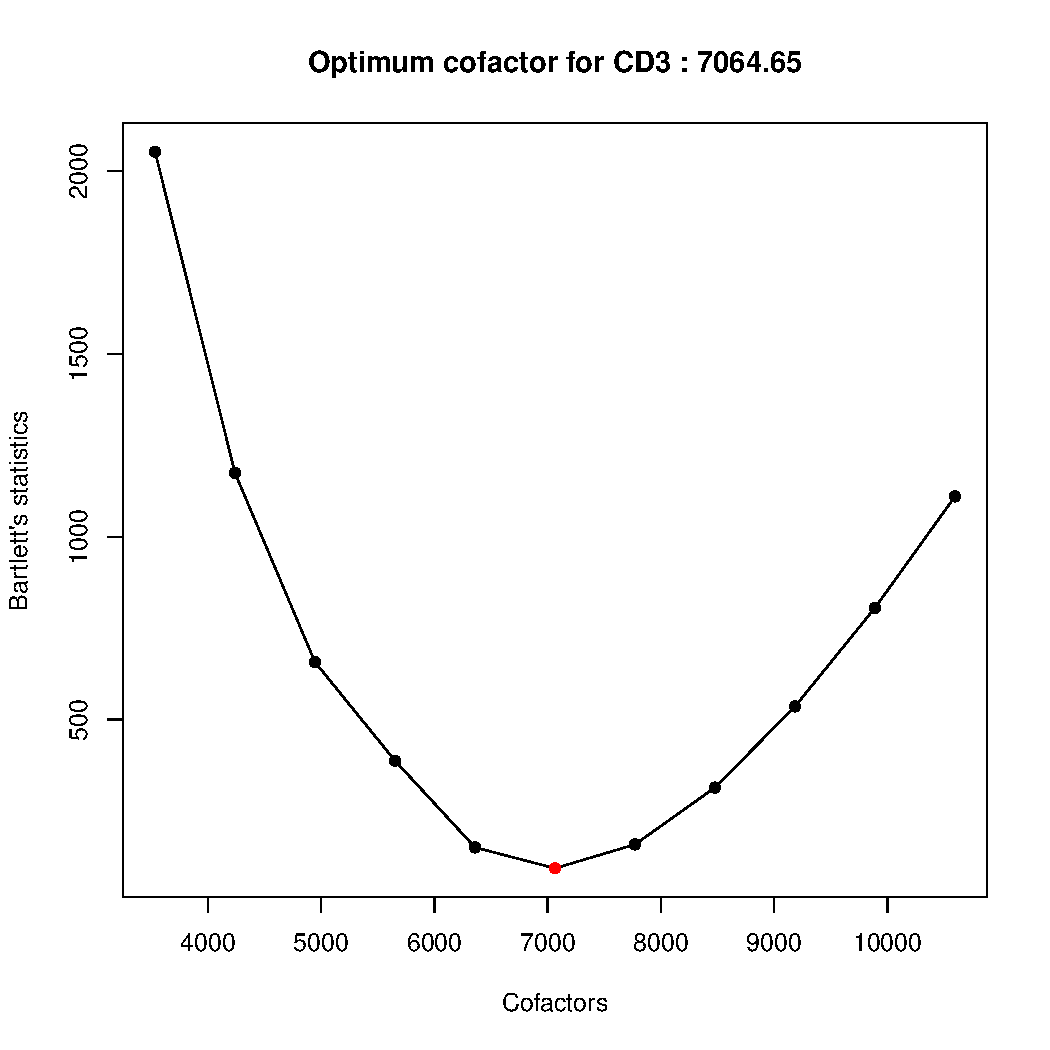
\includegraphics[width=.49\linewidth]{figure/HD-1} 
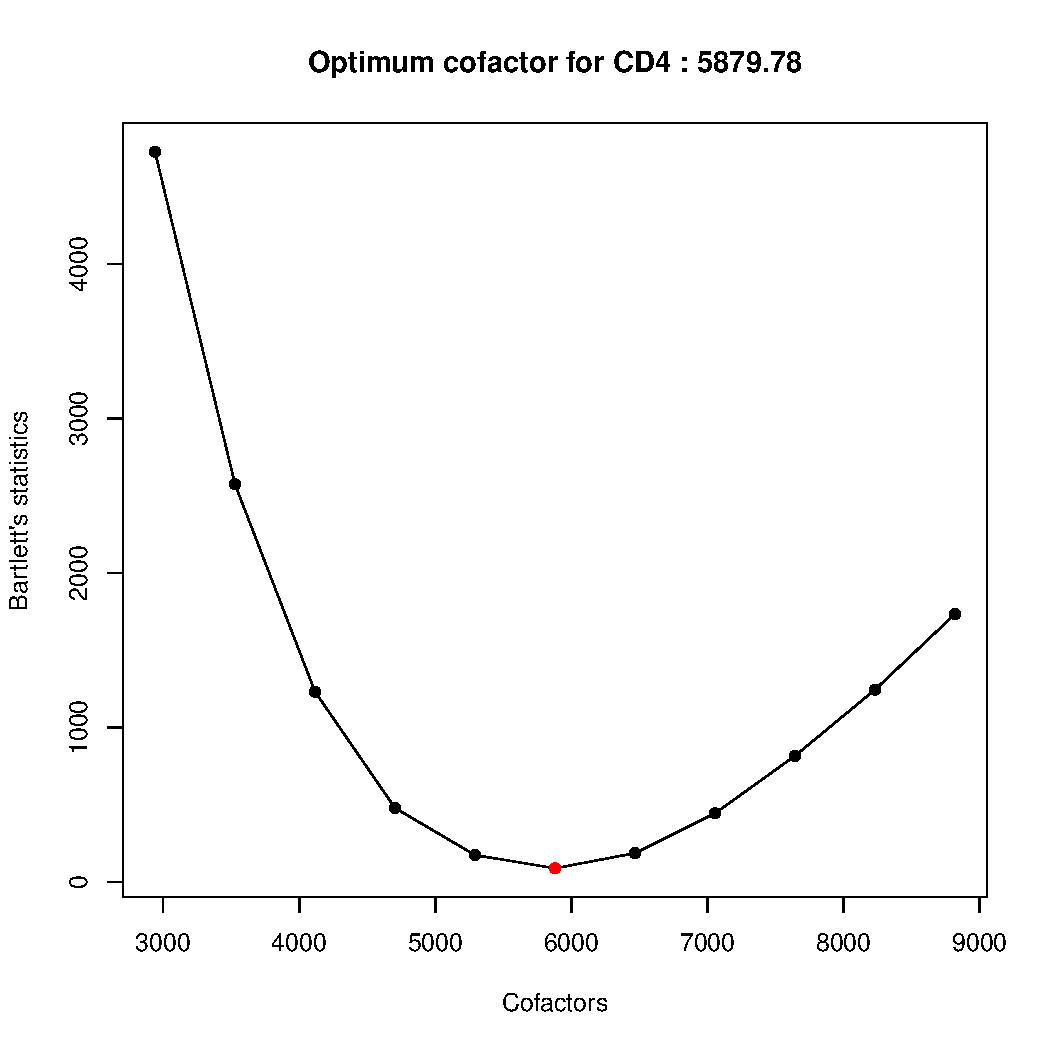
\includegraphics[width=.49\linewidth]{figure/HD-2} \caption[Transforming two fluorescence channels in the HD data]{Transforming two fluorescence channels in the HD data. Bartlett's statistics (Y-axis) is computed from density peaks after data is transformed by different cofactors (X-axis). An optimum cofactor is obtained where Bartlett's statistics is minimum (indicated by red circles).}\label{fig:HD}
\end{figure}


\end{knitrout}


After computing the optimum cofactors for the requested channels, we use \texttt{transFlowVS} function to actually transform the data by asinh transformation with the cofactors.
The density plots show that the variance of populations are relatively stabilized after the transformation.
\begin{knitrout}
\definecolor{shadecolor}{rgb}{0.969, 0.969, 0.969}\color{fgcolor}\begin{kframe}
\begin{alltt}
\hlcom{## transform CD3 and CD4 channels in all samples}
\hlstd{HD.VS} \hlkwb{=} \hlkwd{transFlowVS}\hlstd{(HD,} \hlkwc{channels}\hlstd{=}\hlkwd{c}\hlstd{(}\hlstr{'CD3'}\hlstd{,} \hlstr{'CD4'}\hlstd{), cofactors)}
\end{alltt}
\begin{verbatim}
## Transforming flowSet by asinh function with supplied cofactors.
\end{verbatim}
\begin{alltt}
\hlcom{## density plot (from flowViz package)}
\hlkwd{densityplot}\hlstd{(}\hlopt{~}\hlstd{CD3}\hlopt{+}\hlstd{CD4, HD.VS,} \hlkwc{main}\hlstd{=}\hlstr{"Transfromed CD3 and CD4 channels in HD data"}\hlstd{)}
\end{alltt}
\end{kframe}\begin{figure}
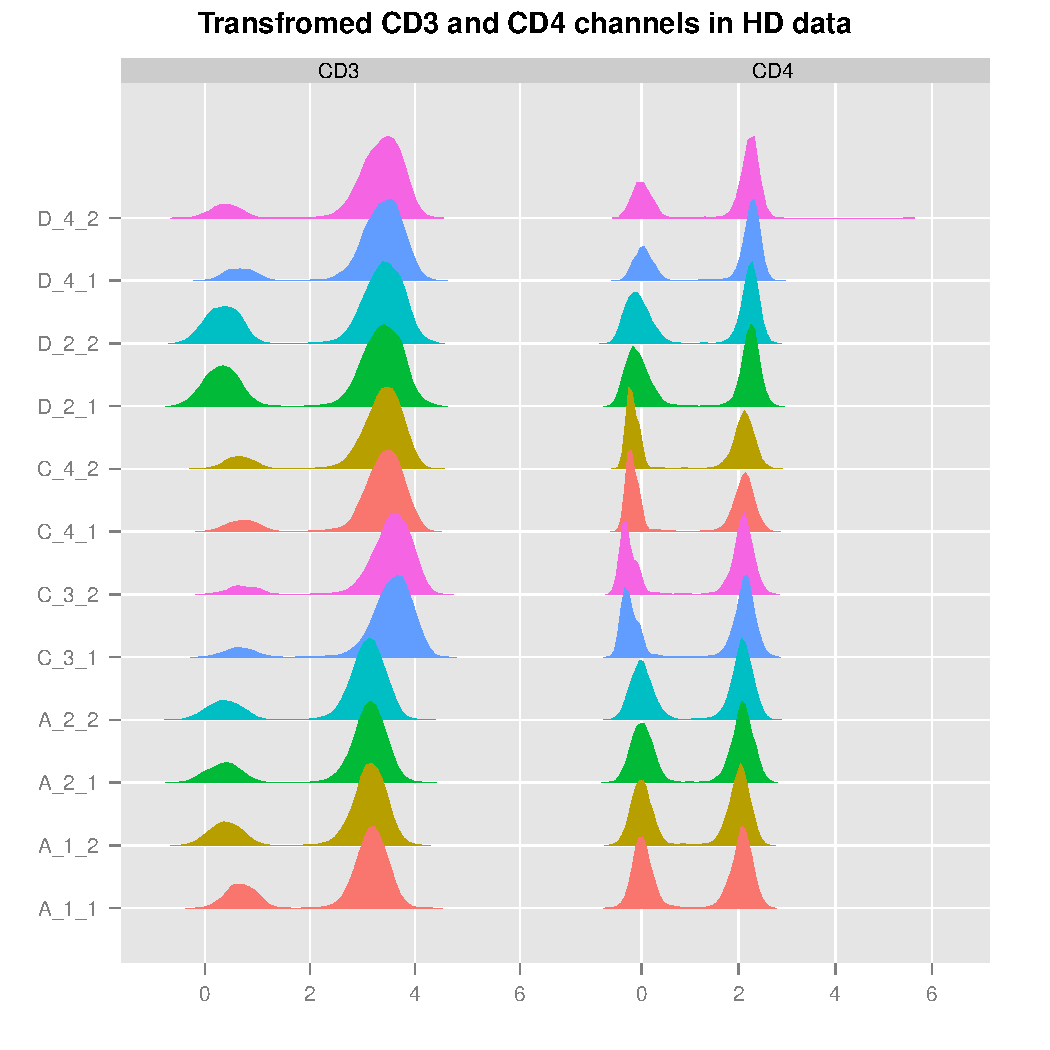
\includegraphics[width=\maxwidth]{figure/densityHD-1} \caption[The density plots after the data is transformed by asins transformation with the optimum cofactors]{The density plots after the data is transformed by asins transformation with the optimum cofactors.}\label{fig:densityHD}
\end{figure}


\end{knitrout}



\subsection{Immune Tolerance Data (ITN)}
We use the Immune Tolerance Network (ITN) dataset from the \Rpackage{flowStats} package in Bioconductor to demonstrate the use of flowVS.
The ITN dataset is collected from 15 patients. It includes 3 patient groups with 5 samples each. 
Each sample was stained using labeled antibodies against CD3, CD4, CD8, CD69 and HLADr.
We identify lymphocytes in each sample of the ITN dataset beforehand by the \texttt{lymphs} function in \Rpackage{flowVS}.


\begin{knitrout}
\definecolor{shadecolor}{rgb}{0.969, 0.969, 0.969}\color{fgcolor}\begin{kframe}
\begin{alltt}
\hlcom{## Example 2: ITN data from flowStats package}
\hlkwd{suppressMessages}\hlstd{(}\hlkwd{library}\hlstd{(flowStats))}
\hlkwd{data}\hlstd{(ITN)}
\hlcom{# identify lymphocytes}
\hlstd{ITN.lymphs} \hlkwb{=} \hlkwd{fsApply}\hlstd{(ITN,lymphs,} \hlkwd{list}\hlstd{(}\hlstr{"FS"}\hlstd{=}\hlkwd{c}\hlstd{(}\hlnum{200}\hlstd{,} \hlnum{600}\hlstd{),}\hlstr{"SS"}\hlstd{=}\hlkwd{c}\hlstd{(}\hlnum{0}\hlstd{,} \hlnum{400}\hlstd{)),} \hlstr{"FSC"}\hlstd{,} \hlstr{"SSC"}\hlstd{,}\hlnum{FALSE}\hlstd{)}
\hlcom{## identify optimum cofactor for CD3 and CD4 channels}
\hlstd{cofactors} \hlkwb{=} \hlkwd{estParamFlowVS}\hlstd{(ITN.lymphs[}\hlnum{1}\hlopt{:}\hlnum{5}\hlstd{],}\hlkwc{channels}\hlstd{=}\hlkwd{c}\hlstd{(}\hlstr{'CD3'}\hlstd{,} \hlstr{'CD4'}\hlstd{))}
\end{alltt}
\begin{verbatim}
## ====================================================================
## Channel  CD3  : Finding optimum cofactor for asinh transformation
## ====================================================================
##           cf range           opt cf    Bartlett's stat      time 
## ====================================================================
## [     0.37,      1.00 ]       0.74          528.32          4.08 
## [     1.00,      2.72 ]       2.62          347.57          3.66 
## [     2.72,      7.39 ]       3.42          324.94          3.34 
## [     7.39,     20.09 ]      18.23          593.21          3.03 
## [    20.09,     54.60 ]      22.01          470.18          3.02 
## [    54.60,    148.41 ]      59.83         2959.76          3.19 
## [   148.41,    403.43 ]     389.22          465.22          3.35 
## [   403.43,   1096.63 ]     691.32          372.03          3.33 
## [  1096.63,   2980.96 ]    1201.64          404.25          3.16 
## [  2980.96,   8103.08 ]    3266.40          456.83          3.17 
## [  8103.08,  22026.47 ]   10134.48          467.90          2.98
## 
##  Optimum cofactor for  CD3  :  3.767 
## ====================================================================
## 
## ====================================================================
## Channel  CD4  : Finding optimum cofactor for asinh transformation
## ====================================================================
##           cf range           opt cf    Bartlett's stat      time 
## ====================================================================
## [     0.37,      1.00 ]       0.85         4591.45          3.03 
## [     1.00,      2.72 ]       2.66         3949.43          3.57 
## [     2.72,      7.39 ]       7.22         1820.98          4.04 
## [     7.39,     20.09 ]      19.38          186.10          2.91 
## [    20.09,     54.60 ]      23.97           97.07          3.01 
## [    54.60,    148.41 ]      59.83          960.44          3.00 
## [   148.41,    403.43 ]     162.62         3854.87          3.02 
## [   403.43,   1096.63 ]     442.06         5078.58          3.03 
## [  1096.63,   2980.96 ]    2261.21         5430.71          2.53 
## [  2980.96,   8103.08 ]    3266.40         5461.95          3.02 
## [  8103.08,  22026.47 ]   11854.06         5450.35          3.14
## 
##  Optimum cofactor for  CD4  :  23.97044 
## ====================================================================
\end{verbatim}
\end{kframe}\begin{figure}
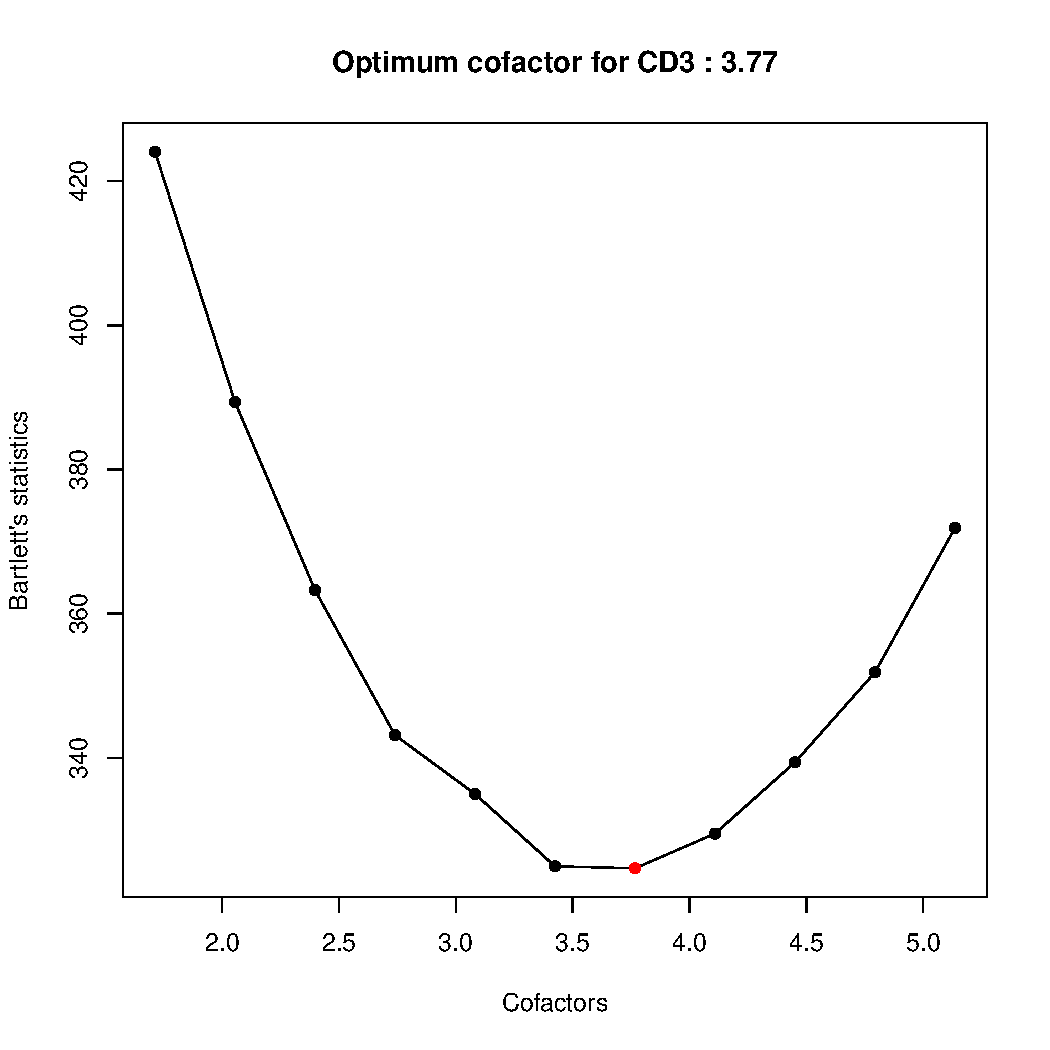
\includegraphics[width=.49\linewidth]{figure/ITN-1} 
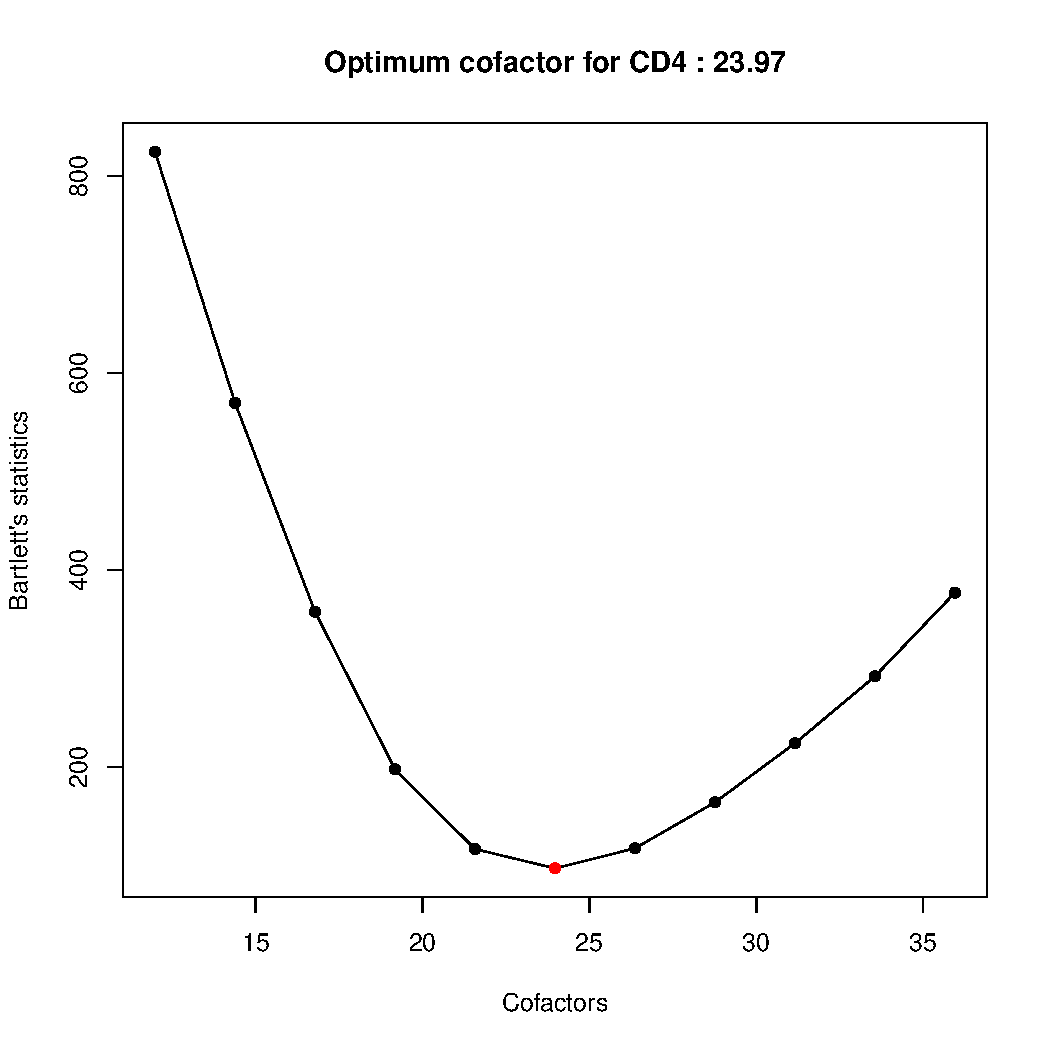
\includegraphics[width=.49\linewidth]{figure/ITN-2} \caption[Transforming two fluorescence channels in the ITN data]{Transforming two fluorescence channels in the ITN data. Bartlett's statistics (Y-axis) is computed from density peaks after data is transformed by different cofactors (X-axis). An optimum cofactor is obtained where Bartlett's statistics is minimum (indicated by red circles).}\label{fig:ITN}
\end{figure}


\end{knitrout}


After computing the optimum cofactors for the requested channels, we use \texttt{transFlowVS} function to actually transform the data by asinh transformation with the cofactors.
The density plots show that the variance of populations are relatively stabilized after the transformation.
\begin{knitrout}
\definecolor{shadecolor}{rgb}{0.969, 0.969, 0.969}\color{fgcolor}\begin{kframe}
\begin{alltt}
\hlcom{## transform CD4 channel in all samples}
\hlstd{ITN.VS} \hlkwb{=} \hlkwd{transFlowVS}\hlstd{(ITN.lymphs,} \hlkwc{channels}\hlstd{=}\hlkwd{c}\hlstd{(}\hlstr{'CD3'}\hlstd{,} \hlstr{'CD4'}\hlstd{), cofactors)}
\end{alltt}
\begin{verbatim}
## Transforming flowSet by asinh function with supplied cofactors.
\end{verbatim}
\begin{alltt}
\hlcom{## density plot (from flowViz package)}
\hlkwd{densityplot}\hlstd{(}\hlopt{~}\hlstd{CD3}\hlopt{+}\hlstd{CD4, ITN.VS,} \hlkwc{main}\hlstd{=}\hlstr{"Transfromed CD3 and CD4 channels in ITN data"}\hlstd{)}
\end{alltt}
\end{kframe}\begin{figure}
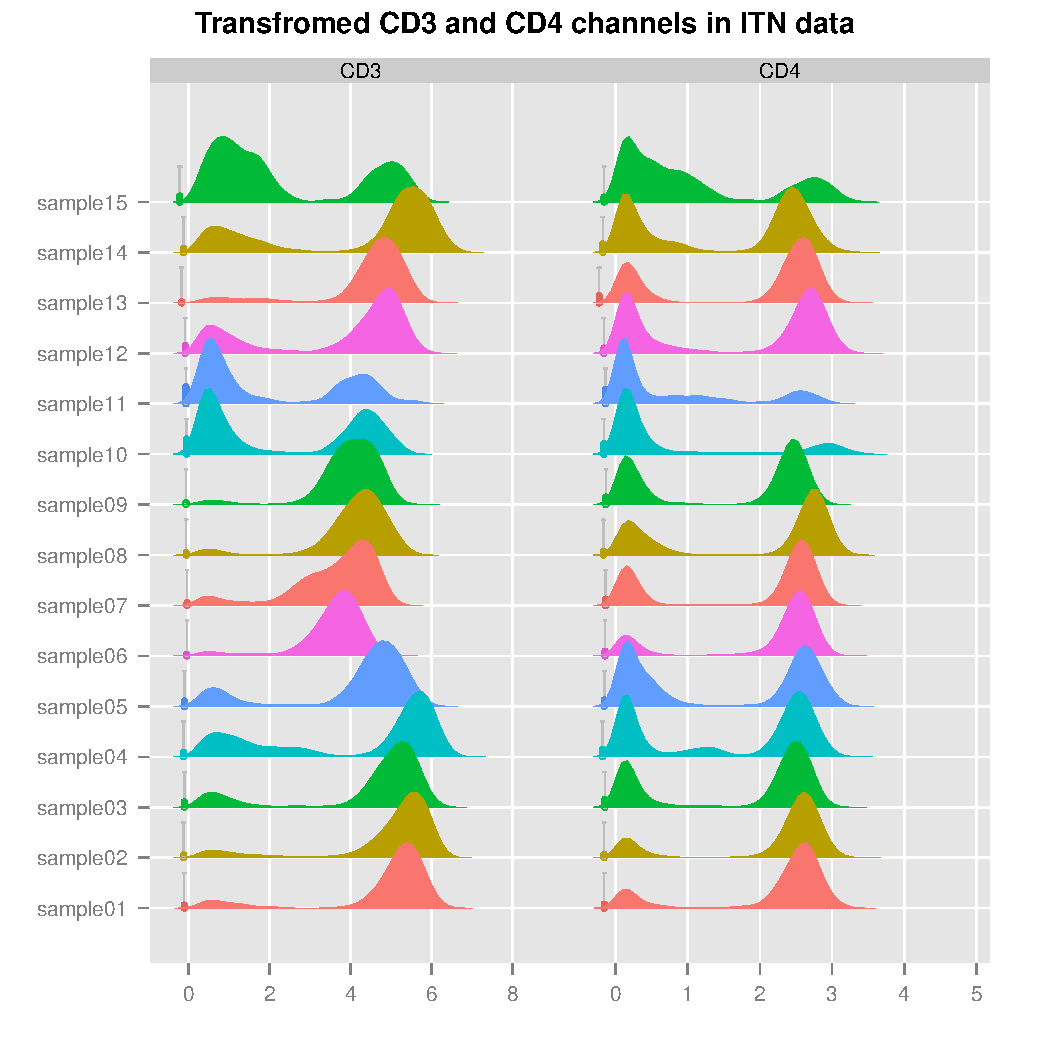
\includegraphics[width=\maxwidth]{figure/densityITN-1} \caption[The density plots after the data is transformed by asins transformation with the optimum cofactors]{The density plots after the data is transformed by asins transformation with the optimum cofactors.}\label{fig:densityITN}
\end{figure}


\end{knitrout}


\section{Variance stabilization in microarray data}
The VS approach based on optimizing Bartlett's statistics can also be used to stabilize variance in microarray data.  
Assume that the expressions of $m$ genes are measured from $N$ samples in a microarray experiment. 
After transforming the data by the asinh function, the mean $\mu_i$ and variance $\sigma^2_i$ of the $i$th gene $g_i$ are computed from the expressions of $g_i$ in all samples.  
We then stabilizes the variances of the genes by transforming data using the asinh function with an optimum choice of cofactor.
Unlike FC, a single cofactor is selected for all genes in microarrays.

The function \texttt{microVS} performs the variance stabilization in microarray data.
This function transforms a microarray data matrix \texttt{z} by \texttt{asinh(z/c)} transformation where \texttt{c} is a normalizing cofactor.
The cofactor is searched in the range \texttt{[cfLow, cfHigh]} and an optimum cofactor is obtained for which the transformed data is variance stabilized.
The optimum cofactor is obtained by minimizing Bartlett's test statistics for homogeneity of variance.

\subsection{Example}
We have applied the \texttt{microVS} to the publicly available Kidney microarray data provided by Huber et al.~\cite{huber2002variance}.
The Kidney data reports the expression of 8704 genes from two neighboring parts of a kidney tumor by using cDNA microarray technology. 
For different values of the cofactor, flowVS transforms the Kidney data with the asinh function and identifies the optimum cofactor by minimizing Bartlett's statistics.
The figure below shows that a minimum value of Bartlett's statistics is obtained when the cofactor is set to $\exp(6)$ ($\sim400$). 
The optimum cofactor is then used with the asinh function to transform the Kidney data.



\begin{knitrout}
\definecolor{shadecolor}{rgb}{0.969, 0.969, 0.969}\color{fgcolor}\begin{kframe}
\begin{alltt}
\hlkwd{suppressMessages}\hlstd{(}\hlkwd{library}\hlstd{(vsn))}
\hlkwd{data}\hlstd{(kidney)}
\hlstd{kidney.microVS} \hlkwb{=} \hlkwd{microVS}\hlstd{(}\hlkwd{exprs}\hlstd{(kidney))} \hlcom{#variance stabilization}
\end{alltt}
\begin{verbatim}
## ====================================================================
## Finding optimum cofactor for asinh transformation
## ====================================================================
## cofactor(log scale)     Bartlett's stat 
## ====================================================================
##          0                  29380.95 
##          1                  26322.83 
##          2                  22577.36 
##          3                  18128.08 
##          4                  13515.48 
##          5                  10073.42 
##          6                   9005.62 
##          7                  10362.98 
##          8                  13159.53 
##          9                  16115.28 
##         10                  18483.08 
## 
##  Optimum cofactor : exp(6) 
## ====================================================================
\end{verbatim}
\end{kframe}
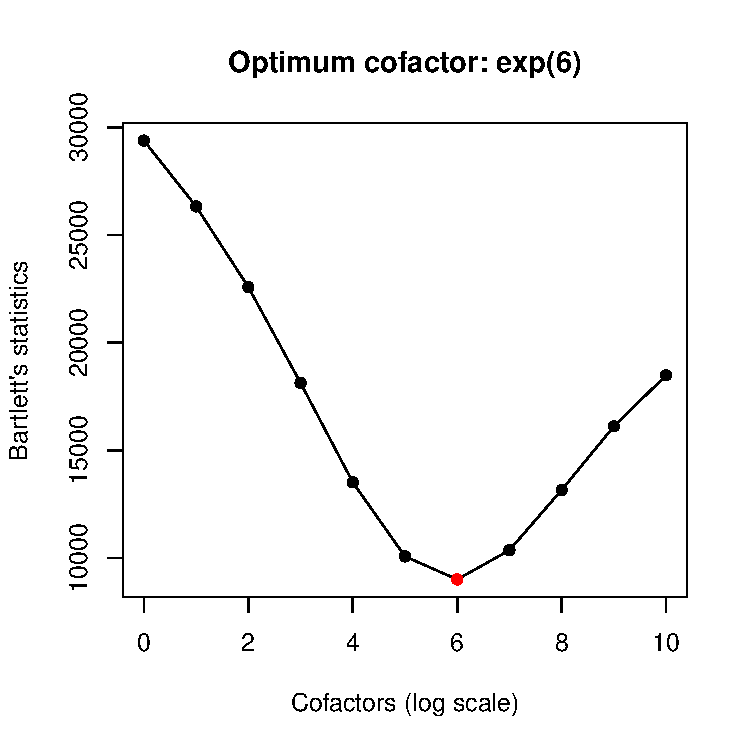
\includegraphics[width=\maxwidth]{figure/microVS-1} 

\end{knitrout}

To take a closer look at the transformed data by \texttt{microVS}, we plot the variances of genes against the ranks of their means.
For this purpose, we included a plotting function \texttt{plotMeanSd} that is modified from the \texttt{meanSdPlot} function in \texttt{vsn} package.
We compare the performance of \texttt{microVS} and \texttt{vsn} in the figures below by using the  \texttt{plotMeanSd} function.
Here, the ranks of means distribute the data evenly along the $x$-axis and thus make it easy to visualize the homogeneity of variances.
We also show the running median estimator of standard deviation by the red lines. 
Both \texttt{vsn} and \texttt{microVS} remove the mean-variance dependence because the red lines are approximately horizontal for both transformations. 
Hence, \texttt{flowVS} performs at least as well as a state-of-the-art approach developed for microarray data.


\begin{knitrout}
\definecolor{shadecolor}{rgb}{0.969, 0.969, 0.969}\color{fgcolor}\begin{kframe}
\begin{alltt}
\hlkwd{suppressMessages}\hlstd{(}\hlkwd{library}\hlstd{(vsn))}
\hlkwd{data}\hlstd{(kidney)}
\hlstd{kidney.vsn} \hlkwb{=} \hlkwd{vsn2}\hlstd{(}\hlkwd{exprs}\hlstd{(kidney))} \hlcom{#variance stabilization by vsn}
\hlkwd{plotMeanSd}\hlstd{(kidney.microVS,} \hlkwc{main}\hlstd{=}\hlstr{"Kidney data: VS by flowVS"}\hlstd{)}
\hlkwd{plotMeanSd}\hlstd{(}\hlkwd{exprs}\hlstd{(kidney.vsn),} \hlkwc{main}\hlstd{=}\hlstr{"Kidney data: VS by vsn"}\hlstd{)}
\end{alltt}
\end{kframe}\begin{figure}

{\centering 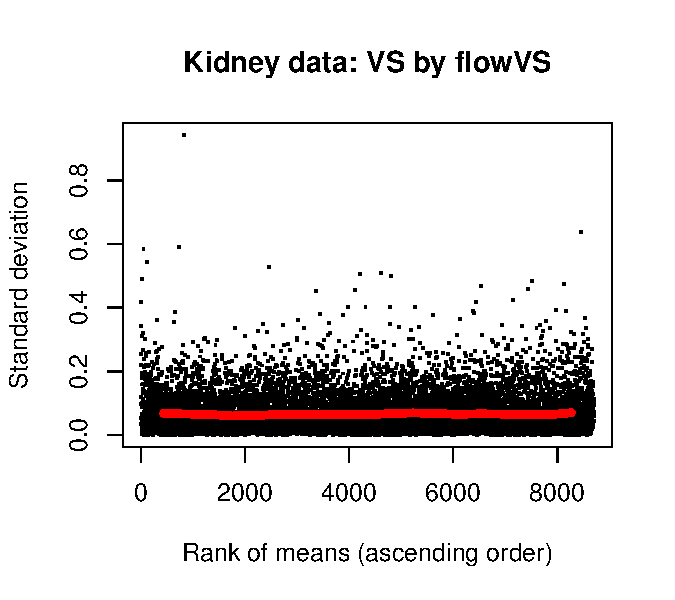
\includegraphics[width=\maxwidth]{figure/vsn-1} 
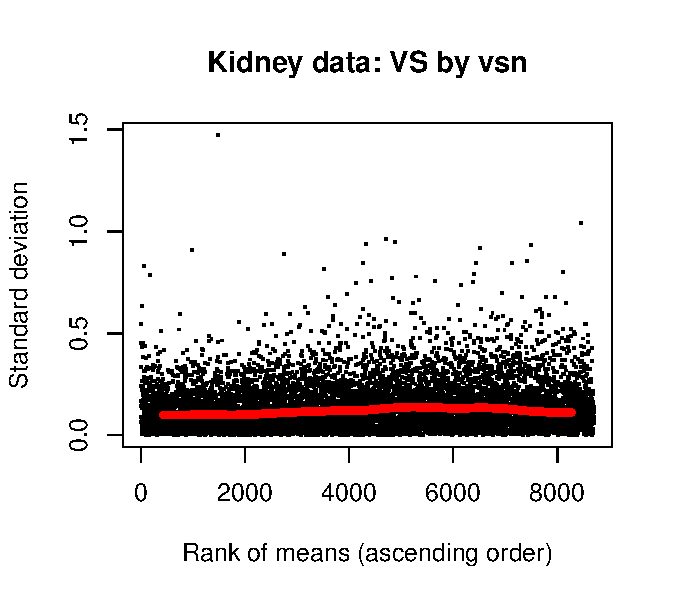
\includegraphics[width=\maxwidth]{figure/vsn-2} 

}

\caption[Variance stabilization of the Kidney microarray data by flowVs and vsn packages]{Variance stabilization of the Kidney microarray data by flowVs and vsn packages.}\label{fig:vsn}
\end{figure}


\end{knitrout}

\newpage
\section{Sessioninfo}
Here is the output of sessionInfo on the system on which this document was compiled:

\begin{kframe}
\begin{alltt}
\hlkwd{toLatex}\hlstd{(}\hlkwd{sessionInfo}\hlstd{())}
\end{alltt}
\end{kframe}\begin{itemize}\raggedright
  \item R version 3.1.1 (2014-07-10), \verb|x86_64-apple-darwin13.1.0|
  \item Locale: \verb|en_US.UTF-8/en_US.UTF-8/en_US.UTF-8/C/en_US.UTF-8/en_US.UTF-8|
  \item Base packages: base, datasets, graphics, grDevices, grid,
    methods, parallel, splines, stats, utils
  \item Other packages: BH~1.55.0-3, Biobase~2.26.0,
    BiocGenerics~0.12.1, cluster~2.0.1, fda~2.4.4,
    flowCore~1.32.2, flowStats~3.24.8, flowViz~1.30.0,
    flowVS~0.99.4, flowWorkspace~3.12.04, gridExtra~0.9.1,
    knitr~1.9, lattice~0.20-31, Matrix~1.1-5, mvoutlier~2.0.6,
    ncdfFlow~2.12.0, RcppArmadillo~0.4.650.1.1, sgeostat~1.0-25,
    vsn~3.34.0
  \item Loaded via a namespace (and not attached): affy~1.44.0,
    affyio~1.34.0, BiocInstaller~1.16.1, chron~2.3-45,
    colorspace~1.2-6, corpcor~1.6.7, data.table~1.9.4,
    DEoptimR~1.0-2, digest~0.6.8, evaluate~0.5.5, formatR~1.1,
    GGally~0.5.0, ggplot2~1.0.1, graph~1.44.1, gtable~0.1.2,
    hexbin~1.27.0, highr~0.4.1, IDPmisc~1.1.17,
    KernSmooth~2.23-14, ks~1.9.4, latticeExtra~0.6-26,
    limma~3.22.1, MASS~7.3-40, misc3d~0.8-4, munsell~0.4.2,
    mvtnorm~1.0-2, pcaPP~1.9-60, pls~2.4-3, plyr~1.8.1,
    preprocessCore~1.28.0, proto~0.3-10, RColorBrewer~1.1-2,
    Rcpp~0.11.5, reshape~0.8.5, reshape2~1.4.1, rgl~0.93.1098,
    Rgraphviz~2.10.0, robCompositions~1.9.0, robustbase~0.92-3,
    rrcov~1.3-8, scales~0.2.4, stats4~3.1.1, stringr~0.6.2,
    tools~3.1.1, XML~3.98-1.1, zlibbioc~1.12.0
\end{itemize}


\bibliographystyle{plain}
\bibliography{flowVS}

\end{document}
